\section{CoDe Design}
\label{sec:design}

% float placed early (cited first in IV-A): column-width schematic, figs/src/fig_tile.html (hand-maintained)
\begin{figure}[t]
  \centering
  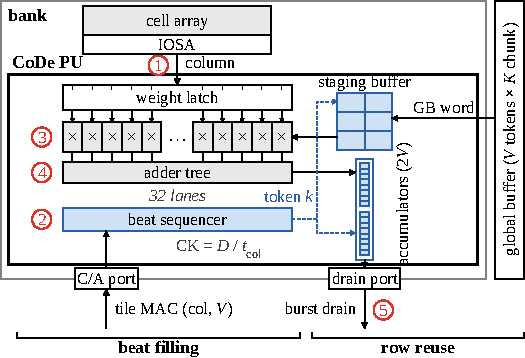
\includegraphics[width=\columnwidth]{figs/fig_tile.pdf}
  \caption{The CoDe PU inside its bank; tint marks the structures CoDe adds or sizes by $V$.}
  \label{fig:tile}
\end{figure}

\subsection{Overview: One Command, Many MAC Beats}
\label{sec:design:overview}

% P:des-tile-mac-overview
CoDe (Command-Decoupled PIM) issues one MAC command per weight column for a tile of $V$ token vectors of a skinny
GEMM, and this single \emph{tile MAC} command carries CoDe's two levers: row reuse (Section~\ref{sec:design:reuse})
and beat filling (Section~\ref{sec:design:beat}). Every command still obeys every DRAM timing parameter: activations,
column reads and refreshes issue exactly as in stock AiM, and only the MAC beats leave the command stream. Both levers
come from the tile, and the tile comes from the global buffer, which CoDe extends from stock AiM's one input vector to
the input vectors of $V$ tokens (Fig.~\ref{fig:tile}, Section~\ref{sec:design:pu}): sharing a row sweep needs $V$
tokens' inputs beside the PU, and filling $D$ beats needs at least $D$ tokens per command. Fig.~\ref{fig:tile} groups
the PU's structures by lever: the staging buffer, the accumulator file and the burst drain carry row reuse, and the
weight latch and the beat sequencer carry beat filling. With both levers, CoDe's useful-MAC utilization $U$ reaches
0.779 on the mobile platform, against stock AiM's 0.179 (Table~\ref{tab:umac}).

% float placed after IV-A (cited first in IV-B); generated by scripts/make_fig_mapping.py (evaluation/dac_2x2 Sec. 2j,
% raw/utrace_run_{stock,core8}.csv), which asserts every number IV-B and IV-C print from the trace
\begin{figure}[t]
  \centering
  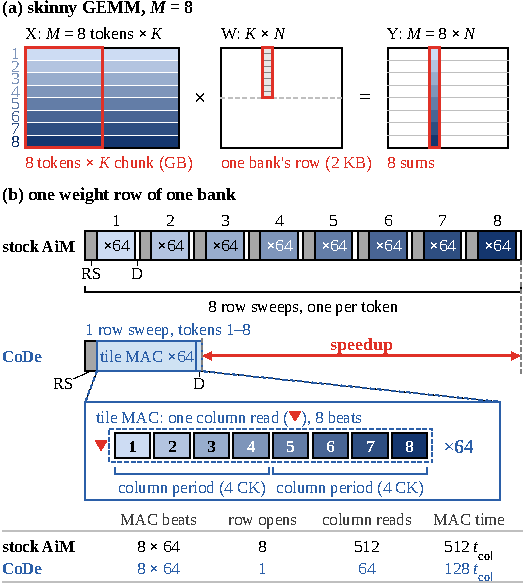
\includegraphics[width=\columnwidth]{figs/fig_mapping.pdf}
  \caption{A skinny GEMM at $M = 8$: (a)~one bank's work per row sweep; (b)~one weight row, stock AiM and CoDe, one
  tile MAC enlarged. RS = row switch; D = drain.}
  \label{fig:mapping}
\end{figure}

\subsection{Row Reuse}
\label{sec:design:reuse}

% P:des-row-reuse
Row reuse answers the non-MAC commands of Section~\ref{sec:bg:cmd}, whose row-switch commands stock AiM pays once per
token. Row reuse lets the $V$ tokens of a tile share one row sweep: the tile MACs sweep the open row's columns once for
all $V$ tokens, so the row-switch commands are paid once per $V$ tokens. Fig.~\ref{fig:mapping}a draws the tile in
GEMM terms at $M = V = 8$: the GB holds the eight tokens' inputs for one chunk of $K$, one bank's open 2\,KB row holds
one output's weights over that chunk, and the tile produces that output's eight sums. In Fig.~\ref{fig:mapping}b,
stock AiM sweeps the weight row once per token and pays a row switch and a drain in each of its eight sweeps, whereas
CoDe pays one row switch for the tile; the row opens fall from eight to one and the column reads from 512 to 64,
because the tile reads each weight from the array once. With $A$ tokens per row sweep, a token pays
$\trow / A + \ttok$ of non-MAC commands per row sweep, plus its share of refresh. The token load/drain commands stay
per token: WRGB writes each token's input chunk into the GB, and the burst drain reads each token's sums once per row
sweep. Row reuse needs the $V$ tokens' inputs next to the PU for the whole row sweep and $V$ partial sums per tile; the
global buffer, the staging buffer and the accumulator file hold them (Section~\ref{sec:design:pu}). The two families
of Section~\ref{sec:bg:walls} tie the tokens of a row sweep to one MAC slot ($A = 2$ and 4 in Table~\ref{tab:umac}),
whereas CoDe sets them by $V$ and leaves the PU's lanes unchanged. The simulated non-MAC time per token thus falls
from stock AiM's 123.39\,ns to CoDe's 22.15\,ns at $V = 8$ on the mobile platform (Table~\ref{tab:umac}) and from
146.17 to 43.51\,ns at $V = 4$ on the edge server.

\subsection{Beat Filling}
\label{sec:design:beat}

% P:des-beat-decouple
Beat filling answers the idle beats of Section~\ref{sec:bg:cmd}, three of a stock MAC slot's four beats, by decoupling
the PU's MAC beats from the command stream. The PU runs its beats at its own clock, $f_\mathrm{PU} = D /
t_\mathrm{col}$, which equals CK on both platforms (Table~\ref{tab:params}), so the PU fits $D$ beats into each column
period whatever the command spacing. A tile MAC holds its column in the PU for $V/D$ column periods, and the next tile
MAC issues $V/D$ periods later. The enlarged tile MAC of Fig.~\ref{fig:mapping}b shows one tile of $V = 8$ tokens at
$D = 4$: one column read feeds eight beats, one per token and four per column period, and each beat adds into its
token's accumulator slot. The bank holds the column for $V/D = 2$ periods, the next tile MAC issues two periods later,
and the tile's partial sums leave in one burst drain after its last column. With $V = D$ the tile fills exactly one
column period, and the MAC commands follow the bank's column rate.

% P:des-beat-slot-factor
Beat filling raises the slot factor from stock AiM's 1/4 to 1, because every beat of a MAC slot computes for one token
of the tile. A PU with the stock multiplier count thus reaches the 4$\times$ ceiling that the wider-PU family reaches
with four times the multipliers. Against the faster-PU family, beat filling saves commands: per token and weight
column, CoDe issues $1/V$ MAC commands, against one for stock AiM and P3-LLM-style and $1/4$ for LP-Spec-style
(Fig.~\ref{fig:timeline}). In the table of Fig.~\ref{fig:mapping}b, the weight row's time in MAC slots falls from 512
to 128 column periods for the same $8 \times 64$ MAC beats. With both levers joined, the weight row takes 738.75\,ns
against stock AiM's 3,250\,ns, 4.40$\times$ shorter, the speedup gap of Fig.~\ref{fig:mapping}b.

\subsection{Tile MAC Command and PU Microarchitecture}
\label{sec:design:pu}

% P:des-command-set
\paragraph{Command set}
CoDe adds two commands to the all-bank interface of AiM-style PIM~\cite{aimjssc} and keeps every other command
(Table~\ref{tab:cmds}). The tile MAC (col, $V$) reads one column from every open bank with the stock MAC command's
timing and tells each PU to run $V$ beats on that column. The burst drain moves a tile's $V$ sums out of every PU in
one burst after the tile's last column. WRGB, TMOD, PREA, ACT16 and WRMAC16 keep their stock definitions, and of these
only the row-switch commands change their count per token.


% P:des-tile-mac-pu
\paragraph{Tile MAC in the PU}
Fig.~\ref{fig:tile} follows one tile MAC through the PU. The tile MAC latches the column that the bank delivers in the
weight latch (\ding{172}). The beat sequencer then steps a token index $k$ from 0 to $V-1$, one beat per CK cycle
(\ding{173}). Beat $k$ multiplies the latched weights by token $k$'s slice from the staging buffer in the lanes (\ding{174}), and the adder
tree adds the products into accumulator slot $k$ (\ding{175}). After the tile's last column, the burst drain moves the
$V$ sums out through the drain port (\ding{176}).

% P:des-storage
\paragraph{Storage}
The global buffer holds the tile's $V$ tokens for one chunk of $K$. On the mobile platform a $K$ chunk holds 2,048 INT8
inputs, 2\,KB per token, so the GB of an eight-token tile holds 16\,KB (Table~\ref{tab:params}); one WRGB burst of 512
writes of 32\,B fills it. The staging buffer next to the lanes is a three-entry queue of 512-bit GB words on the mobile platform, each word
packing two tokens' slices, and a register of $V$ slices on HBM2. The accumulator file holds two sets of $V$ slots per bank, so
one tile's sums drain from one set while the next tile accumulates into the other; an HBM2 PU, which serves two banks,
holds four sets (Table~\ref{tab:params}).

% P:des-tile-size
\paragraph{Tile size}
The tile size $V$ sizes CoDe's storage: the GB holds $V$ tokens' $K$ chunks, the HBM2 staging register holds $V$
slices, and the accumulator file holds two sets of $V$ slots per bank. The lanes, the weight latch, the beat sequencer and the
mobile staging queue keep their size at any $V$. Below $V = D$ the column period paces the PU and beats idle; from
$V = D$ every beat computes, and a larger $V$ cuts only the row-switch term of a token's non-MAC time per row sweep,
about $\trow / V + \ttok$. A weight row takes $\lceil M/V \rceil$ row sweeps, so a last sweep with fewer than $V$
tokens, or any $V > M$, leaves slots idle, and $V$ is sized for the range of $M$ a platform serves. CoDe sets
$V = 2D = 8$ on the mobile platform and $V = D = 4$ on HBM2, where each token needs twice the storage, a 4\,KB $K$
chunk and a 512-bit slice, and one PU serves two banks, so an added slot costs a larger share of the logic
(Section~\ref{sec:eval:ablation}).

% command table (cited first in IV-D): defined in IV-D's right-hand column, so it renders at that column's
% top, opposite Fig. tile; generated by scripts/make_fig_mapping.py
\begin{table}[t]
  \caption{CoDe's commands, counted per token against stock AiM.}
  \label{tab:cmds}
  \centering
  \footnotesize
  \setlength{\tabcolsep}{2.5pt}
  % generated by scripts/make_fig_mapping.py (counts checked on the V = 8 trace, evaluation/dac_2x2 Sec. 2j); do not edit
\begin{tabular}{@{}l>{\raggedright\arraybackslash}p{3.2cm}lcc@{}}
\toprule
Command & Action & Unit & CoDe & Stock \\
\midrule
\emph{tile MAC} (col, $V$) & One column read at the stock MAC timing; $V$ beats on it & column & $1/V$ & 1 \\
\emph{burst drain} & A tile's $V$ sums out in one burst & row sweep & 1 & 1 \\
row switch & TMOD$\times$2, PREA, ACT16 pair, WRMAC16; unchanged & row sweep & $1/V$ & 1 \\
WRGB & GB fill; unchanged & 32\,B of input & 1 & 1 \\
\bottomrule
\end{tabular}

\end{table}

% P:des-pu-clock
\paragraph{PU clock}
CoDe needs a PU clock above the column rate, not one equal to CK, and the tile keeps that clock within the reach of
the DRAM silicon of Section~\ref{sec:bg:depth}. Beat $k$ writes
accumulator slot $k$, so each slot takes one update per tile of $V \ge D$ beats, and the add loop of each slot spans a
column period or more. CoDe's lanes multiply integers, INT8 on the mobile platform and INT4\,$\times$\,INT8 on HBM2,
narrower operands than the BF16 of that section's 1\,GHz multipliers. Each added structure grows with $V$, not with
$D$: CoDe spends its area on storage and keeps the stock multiplier count (Section~\ref{sec:method}).

\subsection{Mapping Skinny GEMMs and Attention}
\label{sec:design:map}

% P:des-mapping
A $K \times N$ weight matrix maps as in stock AiM: the matrix's $N$ output rows spread over the banks, and each row's $K$ weights run along DRAM columns. CoDe cuts the $M$ token rows into tiles of $V$. For each tile the GB holds the tile's
activations for a chunk of $K$; every weight column of the chunk takes one tile MAC command, and the next tile repeats
the row sweep. A tile with fewer than $V$ tokens runs fewer beats on the same commands. Attention runs on the same path
with the KV cache as the weight matrix: $QK^\top$ streams the cached keys against the $M$ query rows, and $PV$ the
cached values against the $M$ rows of probabilities. Speculative decoding verifies $M$ drafted tokens against one
shared KV cache, so speculative-decoding attention is a skinny GEMM as well; a batch reads one cache per request, so batched attention
stays one GEMV per request. The host computes softmax, RoPE and normalisation between the PIM phases.
